%!TEX root = ../main.tex
\chapter{Code and Instructions}
\label{apx:main}

\section{File repository}
\label{FileRep}
The repository with the code to download the system and perform the simulation is available at:
\url{https://github.com/asahicantu/NFT-Thesis}.

 \begin{figure}[!h]
        \centering
        
\includegraphics[width=5cm]{img/QrCode.png}
        \caption{Qr Code which will redirect to the Github Project stated in \ref{FileRep}}.
        \label{fig:QRCode}
\end{figure}

\section{Instructions to run the code}
To run the project follow the following steps:

\subsection{Prerequisites}
A Linux operating system or bash scripting shell is required.
On a windows machine the usage of \ac{WSL} (any Linux distribution) can help to run the project
Docker Desktop installed (if using Windows with \ac{WSL} make sure the option 'Use WSL 2 Based engine' or similar is selected).

\subsection{Run the application}
\begin{enumerate}
    \item Clone the repository
    \begin{lstlisting}[language=sh]
    git clone https://github.com/asahicantu/NFT-Thesis.git
    \end{lstlisting}
    \item Move to the repository's directory and then to the network directory
    \begin{lstlisting}[language=sh]
    cd NFT-Thesis/network
    \end{lstlisting}
    \item Enable execution mode for all .sh (shell scripting files)
    \begin{lstlisting}[language=sh]
    find . -name "*.sh" -exec chmod +x {} \;
    \end{lstlisting}
    \item Run the network infrastructure
    \begin{lstlisting}[language=sh]
    ./network start
    \end{lstlisting}
    \item Confirm no error occurred
     \begin{figure}[!h]
        \centering
        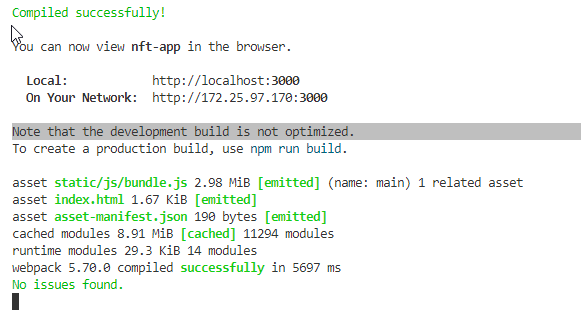
\includegraphics[width=10cm]{img/Client_Shell.png}
        \caption{Network shell showing successful run}.
        \label{fig:Network_Shell}
    \end{figure}
    \item Run server application in a different terminal
    \begin{lstlisting}[language=sh]
    cd ../web/server && npm install && npm run dev`
    \end{lstlisting}
    \item Confirm no error occurred
     \begin{figure}[!h]
        \centering
        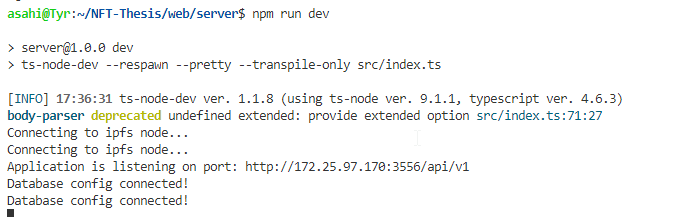
\includegraphics[width=10cm]{img/Server_Shell.png}
        \caption{Server shell showing successful run}.
        \label{fig:Server_Shell}
    \end{figure}
    \item Run web application in a different terminal
    \begin{lstlisting}[language=sh]
    cd ../client && npm install && npm run start`
    \end{lstlisting}
     \item Confirm no error occurred
     \begin{figure}[!h]
        \centering
        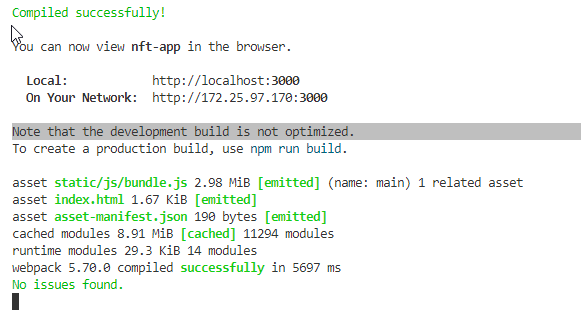
\includegraphics[width=10cm]{img/Client_Shell.png}
        \caption{Client shell showing successful run}.
        \label{fig:Client_Shell}
    \end{figure}
    \item Open the application in a web browser by using:
    \url{http://localhost:3000}.
    \item Confirm all steps were properly followed and no error occurred
     \begin{figure}[!h]
        \centering
        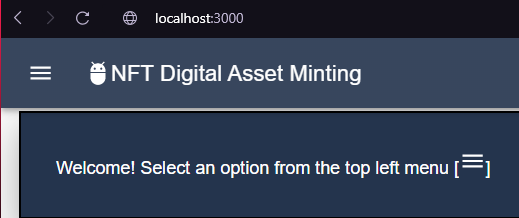
\includegraphics[width=10cm]{img/UI_MAIN.png}
        \caption{Main UI Page should be visible}.
        \label{fig:UI_MAIN}
\end{figure}

\end{enumerate}